\documentclass[11pt]{article}

\usepackage[review]{acl}
\usepackage{times}
\usepackage{latexsym}
\usepackage[T1]{fontenc}
\usepackage[utf8]{inputenc}
\usepackage{microtype}
\usepackage{amsmath,amssymb}
\usepackage{graphicx}
\usepackage{booktabs}
\usepackage{xcolor}

\title{Tool-Intent Stabilization Is Operationalization-Dependent:\\
A Cautionary Measurement Study of Streaming Retrieval-Augmented Generation}
\author{Anonymous}

% ===================================================================== %
% RESULTS MACROS — populated from results/*.summary.json (see fill note) %
% ===================================================================== %
% Workload
\newcommand{\nTotal}{2706}
\newcommand{\nSplitZero}{1371}
\newcommand{\nGroundPct}{35.4\%}      % groundable %
\newcommand{\nRetrPct}{21.3\%}        % gold retrieved in top-k at some prefix (k=3) %
\newcommand{\nFallbackPct}{78.7\%}    % fallback (t_sc) population = 100% - nRetrPct %
% RQ1 (k=3)
\newcommand{\phiScMean}{0.67}
\newcommand{\phiScMed}{0.73}
\newcommand{\phiSufMean}{0.26}
\newcommand{\phiSufMed}{0.14}
% Grounding-PRECISION correction (experiments/grounding_precision.py): restrict to
% questions whose gold answer grounds specifically (gold set <= 5% of passages), so a
% random top-3 hits gold <= ~15% of the time. Bounds the over-grounding of short/
% ubiquitous answers that the exact/fuzzy arms share. n=58.
\newcommand{\phiSufClean}{0.44}      % phi_suf mean, precisely-grounded
\newcommand{\phiSufCleanMed}{0.35}   % phi_suf median, precisely-grounded
\newcommand{\nCleanGround}{58}       % precisely-grounded subset size
\newcommand{\tSufOneAll}{49\%}       % t_suf==1 share, all retrieved-gold
\newcommand{\tSufOneClean}{14\%}     % t_suf==1 share, precisely-grounded
\newcommand{\volMean}{0.52}
\newcommand{\volSharePct}{20.9\%}
% RQ2 (central cell L=600, delta=3, theta=0.8)
\newcommand{\streamPct}{73.9\%}
% RQ3 (paired replay of the SAME 60 questions at two tool latencies)
\newcommand{\rqThreeN}{60}
\newcommand{\measSaved}{1122}        % L=600 measured mean %
\newcommand{\hPred}{590}             % L=600 H mean %
\newcommand{\rhoLsix}{+0.14}         % Spearman(H, measured) at L=600 %
\newcommand{\measSavedLk}{1457}      % L=1000 measured mean %
\newcommand{\hPredLk}{950}           % L=1000 H mean %
\newcommand{\rhoLk}{+0.12}           % Spearman(H, measured) at L=1000 %
\newcommand{\nSatLsix}{59}           % L=600: queries pinned at H=600 (of 60) %
\newcommand{\nTailLk}{7}             % L=1000: queries below the H cap (of 60) %
% RQ2 population split (central cell L=600, delta=3, theta=0.8)
\newcommand{\streamSufPct}{95.2\%}   % streamable among retrieved-gold, using t_suf (n=292) %
\newcommand{\streamScPct}{68.1\%}    % streamable among fallback, using t_sc (n=1079) %
% RQ4 significance
\newcommand{\kwAllH}{17.0}           % Kruskal-Wallis H, all 8 types %
\newcommand{\kwAllP}{0.017}
\newcommand{\kwBigH}{13.9}           % Kruskal-Wallis H, 5 classes with n>=10 %
\newcommand{\kwBigP}{0.008}
\newcommand{\epsSq}{0.06}            % KW rank effect size eps^2 = H/(n-1), all 8 types; stats.py %
\newcommand{\epsSqBig}{0.05}         % KW eps^2 = H/(n-1), 5 classes with n>=10; stats.py %
% Arora et al. per-stage latencies used to calibrate RQ3 (ms)
\newcommand{\qgenMs}{590}            % query generation %
\newcommand{\fuseMs}{2520}           % fuse/reflect %
% Robustness: relaxed (fuzzy bag-of-content-token) grounding arm, k=3
\newcommand{\groundFuzzyPct}{43.3\%} % groundable under fuzzy (vs 35.4 exact) %
\newcommand{\retrFuzzyPct}{24.4\%}   % retrieved-gold under fuzzy (vs 21.3 exact) %
\newcommand{\phiSufFuzzy}{0.281}     % phi_suf mean under fuzzy (vs 0.264 exact) %
\newcommand{\nSetFuzzy}{20}          % 'set' support under fuzzy (vs 2 exact) %
% Robustness: t_sc-population mis-fire replay (L=600, delta=3) vs the suf replay
\newcommand{\negRateSuf}{1.7\%}      % net-negative-saving rate, retrieved-gold pop %
\newcommand{\negRateSc}{1.7\%}       % net-negative-saving rate, t_sc fallback pop %
\newcommand{\phiScReplay}{0.68}      % mean phi of the t_sc replay sample %
% Robustness: dense-retriever arm (all-MiniLM-L6-v2, cosine, k=3, split 0)
\newcommand{\retrDensePct}{26.5\%}   % retrieved-gold, dense (vs 21.3 BM25) %
\newcommand{\phiScDense}{0.85}       % phi_sc mean, dense (vs 0.67) %
\newcommand{\phiSufDense}{0.31}      % phi_suf mean, dense (vs 0.26) %
\newcommand{\phiSufDenseMed}{0.22}   % phi_suf median, dense (vs 0.14) %
\newcommand{\rhoDenseType}{0.79}     % Spearman(BM25,dense) over phi_suf type ranking %
% ---- Global-corpus arm (Paper 1 v2 spine). Sources named per line. ----
% phi_suf dose-response + retriever-generality (gold-guaranteed subsamples)
\newcommand{\phiSufGnqK}{0.571}      % NQ gold+1k median phi_suf; results/global/confirm/nq_bm25_1000.summary.json
\newcommand{\phiSufGnqTenK}{0.625}   % NQ gold+10k median; nq_bm25_10000.summary.json
\newcommand{\phiSufGnqOneM}{0.75}    % NQ ~1M-prefix median; nq_tsuf.1m.summary.json
\newcommand{\phiSufGfiqaBm}{0.636}   % FiQA gold+10k BM25 median; fiqa_bm25_10k.summary.json
\newcommand{\phiSufGfiqaDe}{0.625}   % FiQA gold+10k dense median; fiqa_dense_10k.summary.json
\newcommand{\tSufOneGnqOneM}{0.7\%}  % NQ ~1M t_suf==1 rate; nq_tsuf.1m.summary.json
\newcommand{\tSufOneGfiqaBm}{2.8\%}  % FiQA 10k BM25 t_suf==1; fiqa_bm25_10k.summary.json
\newcommand{\nGfiqaBm}{364}          % FiQA 10k BM25 groundable n; fiqa_bm25_10k.summary.json
\newcommand{\nGfiqaDe}{481}          % FiQA 10k dense groundable n; fiqa_dense_10k.summary.json
% L-dependent headroom: streamable fraction, delta=3, theta=0.8 (full corpora)
% per-question CRAG (v1): results/global/headroom/perq_crag.json
\newcommand{\sfPqSix}{73.9\%}        % L=600  (matches v1 \streamPct)
\newcommand{\sfPqFifteen}{54.5\%}    % L=1500
\newcommand{\sfPqTwentyfive}{39.2\%} % L=2500
% global NQ ~1M: results/global/headroom/nq_1m.json
\newcommand{\sfNqSix}{58.6\%}        % L=600
\newcommand{\sfNqFifteen}{27.2\%}    % L=1500
\newcommand{\sfNqTwentyfive}{9.2\%}  % L=2500
% global FiQA full ~57k: results/global/headroom/fiqa_full.json
\newcommand{\sfFiqaSix}{67.6\%}      % L=600
\newcommand{\sfFiqaFifteen}{48.8\%}  % L=1500
\newcommand{\sfFiqaTwentyfive}{30.8\%} % L=2500
% ===================================================================== %

\begin{document}
\maketitle

\begin{abstract}
Streaming Retrieval-Augmented Generation (Streaming RAG) hides tool latency by
issuing retrieval queries in parallel with the user's still-arriving input, before
the utterance is complete. Speculation can only help, though, when the correct
query becomes determinable before the user stops speaking or typing---a property of
the query, not the system. We name and measure this property,
\textbf{tool-intent stabilization} (TIS): the point in the input stream at which a
speculative query's retrieval converges on the answer-bearing result.

The measured value of TIS depends critically on the retrieval corpus.
Against the per-question candidate pool that CRAG ships, stabilization looks early
(median $\phi_{\mathrm{suf}}=\phiSufMed$); against a realistic global corpus it is
late (median up to $\phiSufGnqOneM$ on NQ at ${\sim}1$M documents), grows later
with corpus size, and holds for both sparse and dense retrieval (FiQA: BM25
$\phiSufGfiqaBm$, dense $\phiSufGfiqaDe$).

This corpus-dependence has a direct consequence for the hideable-latency headroom,
and the gap grows with tool latency. At a large tool latency ($L{=}2500$ ms, the
regime streaming RAG targets) the streamable fraction falls from \sfPqTwentyfive{}
(per-question corpus) to \sfNqTwentyfive{} (global NQ)---whereas at small tool
latency ($L{=}600$ ms) long queries still capture meaningful headroom in both
conditions.

The TIS framework ($t_{\mathrm{sc}}$, $t_{\mathrm{suf}}$, $\phi$, and the bound
$H$) is sound; the caution is to measure TIS against the corpus the deployed system
retrieves over. On the CRAG benchmark (\nSplitZero{} validation questions) we
(i) characterize how stabilization is distributed; (ii) derive a model-agnostic
bound $H$ on the latency hideable behind the remaining input; (iii) validate $H$
against a working pipeline; and (iv) identify query properties that predict early
versus late stabilization. The study needs no model training and runs on commodity
CPU hardware.
\end{abstract}

\section{Introduction}
Tool-augmented dialogue systems increasingly rely on external retrieval to remain
factual, but tool calls add latency that disrupts conversational flow. Streaming
RAG~\cite{arora2025streamrag} addresses this by predicting and issuing tool
queries in parallel with the user's still-arriving input, then reflecting
on whether retrieved results suffice. The approach reports sizable accuracy and
latency improvements and is modality-agnostic, applying equally to typed input.

The reported latency benefit, however, is an aggregate over a benchmark. It
leaves a basic question unanswered: \textbf{for which queries can speculation
help at all, and by how much?} The answer is not a property of the model, the
retriever, or the speech stack. It is a property of where, within an utterance,
the information that determines the tool query first appears. If the
decisive term arrives last (``who makes the console called the
\emph{PlayStation}''), no early speculative query can retrieve the right evidence,
and the latency win collapses to zero regardless of system quality. If the
decisive term arrives early, almost the entire tool latency can be hidden behind
the remaining input.

We initially measured tool-intent stabilization against the per-question candidate
pool that CRAG ships with each query, and that measurement made stabilization look
early (median $\phi_{\mathrm{suf}}=\phiSufMed$).  Measuring instead against a
realistic global corpus---the corpus the deployed system actually retrieves
over---reveals that early picture to be largely an artifact of the
per-question pool: stabilization is in fact \emph{late} (median $\phi_{\mathrm{suf}}$
up to $\phiSufGnqOneM$ on NQ at ${\sim}1$M documents), grows later with corpus
size, and holds for both sparse and dense retrieval.  This corpus-dependence is
the finding this paper is organized around.

We study this directly. By characterizing tool-intent stabilization as a
measurable, query-intrinsic quantity, we obtain: (i) a model-agnostic
\emph{aggregate} bound $H$ on the share of tool latency that can be hidden behind
ongoing input, computable \emph{before} any system is built, but
\emph{operationalization-sensitive}---the corpus the bound is evaluated on
determines how optimistic or conservative it is; (ii) a measurement caution
backed by global-corpus evidence---dose-response across corpus sizes, two
benchmarks (NQ and FiQA), and two retriever families (BM25 and dense)---showing
that per-question pools substantially over-estimate real-world headroom, and that
headroom shrinks as tool latency grows; (iii) a principled account of the failure
mode (late stabilization) and a coarse build/skip signal for whether a learned
trigger is worth its compute cost; and (iv) results that transfer across text and
speech because the quantity is modality-agnostic.  Our contribution is
measurement and analysis rather than a new system.

\section{Background and Related Work}
Retrieval-Augmented Generation~\cite{lewis2020rag} grounds generation in
retrieved evidence; dense passage retrieval~\cite{karpukhin2020dpr} and the
sparse BM25 model~\cite{robertson2009bm25} are the standard retrieval backbones.
Streaming RAG~\cite{arora2025streamrag} adds a speculative dimension: a
\emph{Trigger} decides when to fire a tool query from a partial utterance,
multiple speculative \emph{Threads} run in parallel, and a \emph{Reflector}
judges whether results suffice. The idea is closely related in spirit to
speculative decoding~\cite{leviathan2023speculative}, which hides latency by
doing work that may be discarded; here the discarded work is a premature tool
call. Our analysis is orthogonal to the system: we quantify the headroom that any
such system can exploit, set by the query alone. Two literatures tell us why such
headroom should exist and how to measure when a prefix is safe to act on.

\subsection{Incremental comprehension and anticipation}
Why expect tool intent to settle before a query is complete? Human comprehension
already works this way. That the referential
intent of an utterance is fixed incrementally---often well before the utterance
ends---is among the most robust findings in psycholinguistics.
\citet{altmann1999incremental} showed that a verb such as ``eat'' directs
anticipatory attention to edible objects before they are named, so partial input
already restricts what can follow. \citet{kamide2003timecourse} extend this
cross-linguistically: in head-final Japanese, case-marked pre-verbal arguments let
comprehenders anticipate a forthcoming argument even before the verb (the head) is
heard---\emph{pre-head} anticipation~\cite{kamide1999prehead}. This is the human
analogue of firing a tool query from a prefix: \emph{where} the disambiguating
cue sits---varying with word order and case morphology---governs how early intent
stabilizes.

\subsection{Stabilization over a growing prefix}
If comprehension fixes intent early, an engineered system faces the dual problem:
deciding when a prediction over a growing input prefix becomes safe to commit. This
is the central question of \emph{simultaneous} and \emph{incremental} NLP. Simultaneous machine
translation must decide, token by token, whether enough source has arrived to emit
output: wait-$k$ and prefix-to-prefix policies~\cite{ma2019stacl} and learned
read/write agents~\cite{gu2017simultaneous} trade latency against the risk of
committing before the disambiguating word arrives---precisely our $L$-versus-residual
tension. \citet{grissom2014dont} cast the same problem as an agent that waits until
it can confidently predict the sentence-final verb before committing; its failure
mode, premature commitment forcing revision, is exactly what our volatility $V$
records. Closest to our measurement is incremental spoken language understanding:
\citet{devault2011incremental} build a meaning frame from partial ASR and quantify
understanding as a function of prefix length, and the incremental-unit
framework~\cite{schlangen2011incremental} formalizes the same prefix-monotonicity
and revision concerns. These efforts target a \emph{closed} intent or dialogue-act
ontology. Our contribution is to port the lens to \emph{tool/retrieval} intent over
an open-world knowledge benchmark: rather than learning a commit policy, we
\emph{measure} the query-intrinsic point at which the retrieval target stabilizes,
which upper-bounds what any such policy could hide.

\section{Problem Formalization}
Let a query $Q$ be a word sequence $q_{1:n}$ of length $n$ words, and let $q_{1:t}$
denote the prefix of the first $t$ words (we measure stabilization in words
throughout, matching the whitespace tokenization used by both the retriever and
the input-cadence model below). Let $R$ be a retriever returning a
ranked document list; write $d_t = \mathrm{top\text{-}1}(R(q_{1:t}))$ for the top
document retrieved from the prefix, $d_n$ for the full-query top document, and
$d^\star$ for the gold answer-bearing document.

\paragraph{Self-consistency stabilization $t_{\mathrm{sc}}$.} the smallest $t$
such that for all $s \in \{t, \ldots, n\}$, $d_s = d_n$: every prefix from $t$
onward retrieves the same top document as the full query.

\paragraph{Sufficiency stabilization $t_{\mathrm{suf}}(q; C)$.} the smallest $t$
such that $d^\star \in \mathrm{top\text{-}}k(R(q_{1:t}; C))$: retrieval over
corpus $C$ already surfaces the gold evidence in the prefix. This is the
operationally meaningful notion, since the full query itself may retrieve
imperfectly. The corpus $C$ is an explicit parameter: our v1 results are
$t_{\mathrm{suf}}(\cdot;\,C_{\mathrm{perq}})$, where $C_{\mathrm{perq}}$ is
CRAG's per-question candidate pool; the global-corpus arm reports
$t_{\mathrm{suf}}(\cdot;\,C_{\mathrm{global}})$ over a realistic open-domain
index. Because $C_{\mathrm{perq}}$ is far smaller and topically filtered,
$t_{\mathrm{suf}}(\cdot;\,C_{\mathrm{perq}})$ systematically under-estimates
how late stabilization actually occurs in deployment; all sufficiency results
in this paper specify which corpus is in use.

\paragraph{Stabilization fraction $\phi = t^\star/n \in (0,1]$,} reported for both
$t_{\mathrm{sc}}$ and $t_{\mathrm{suf}}$. Lower $\phi$ means earlier stabilization
and more headroom to hide latency.

\paragraph{Stabilization volatility $V$,} the number of top-1 changes occurring
\emph{after} $d_n$ is first reached. High $V$ signals early-commit risk: a
confident-looking early result that a later token would overturn.

\paragraph{Hidden latency.}
\begin{equation}
H(Q; L, \delta) = \min\!\Big(L,\; \max\!\big(0,\; \tfrac{n - t^\star}{\delta}\big)\Big),
\end{equation}
where $L$ is tool latency (ms) and $\delta$ is the input cadence in words per
second, so that $(n-t^\star)/\delta$ is the residual input time (in seconds, scaled
to ms) still to arrive after the query has stabilized. $H$ is the portion of tool
latency that completes behind the user's remaining input. It bounds the
\emph{input-hideable} component of the per-query perceived-latency saving---not the
total saving, since a real pipeline can additionally overlap other costs (\S5.4).
A slower cadence (smaller $\delta$) lengthens the residual and so raises $H$ when
tool latency is the larger term.

\paragraph{Streamable.} $\mathrm{Streamable}(Q; L, \delta, \theta)$ holds iff
$H \geq \theta L$ for a coverage threshold $\theta$ (e.g.\ $\theta=0.8$ hides at
least 80\% of tool latency). The streamable fraction of a workload is the central
deployment-relevant statistic.

\paragraph{Research questions.} We address four pre-registered questions.
\textbf{RQ1} asks how $\phi$ is distributed across queries; under the
per-question operationalization ($C_{\mathrm{perq}}$) the distribution is
right-skewed with an early-stabilizing mass and a thin late tail---and a central
question is whether that early mass is intrinsic to the queries or an artifact of
the small, topically-filtered corpus, which the global-corpus arm answers.
\textbf{RQ2} asks what fraction of queries admit latency hiding as $L$, $\delta$,
and $\theta$ vary; we expect that for large $L$ the binding constraint is the
residual input time $(n-t^\star)/\delta$, so a \emph{slower} cadence
paradoxically \emph{raises} the streamable fraction.
\textbf{RQ3} asks whether the $H$ bound matches a working pipeline.
\textbf{RQ4} asks which query features predict early vs.\ late stabilization; we
expect question type to be the dominant signal, with simple lookups stabilizing
earlier than multi-hop or aggregation queries.
We address RQ1--RQ4 in \S5 and include top-$k$ and dense-retriever robustness
arms (Table~\ref{tab:topk}, \S\ref{sec:robust}) as sensitivity checks. A
cross-linguistic condition is left to future work. We report
disconfirmations alongside confirmations: RQ2 is confirmed, but the RQ1
distribution is right-skewed rather than bimodal (\S5.1), and the RQ4 ordering
is governed by entity position rather than reasoning complexity (\S5.2).

\section{Method}\label{sec:method}
\paragraph{Data.} We use CRAG, the Comprehensive RAG
Benchmark~\cite{yang2024crag}, Task 1\&2 dev set: \nTotal{} questions, of which
\nSplitZero{} are the validation split we analyze. Each question carries up to
five retrieved web pages, a gold answer (plus alternates), and a question-type
label.

\paragraph{Grounding $d^\star$.} CRAG provides no gold-\emph{passage} label, only
gold answer strings. We derive $d^\star$ by grounding the normalized gold
answer(s) into passage text: substring match for multi-token answers, and
word-boundary match for single-token answers, over the answer and its alternates.
Questions whose answer is never a literal span (false-premise, ``I don't know'',
and many aggregation/dynamic answers) are \emph{ungroundable} and excluded from
$t_{\mathrm{suf}}$; we report the groundable rate explicitly. Because
$t_{\mathrm{sc}}$ requires no grounding, we report it as a grounding-free
robustness check alongside $t_{\mathrm{suf}}$.

String grounding is a recall-oriented heuristic and can produce false positives.
A single-token gold answer (a year, a number, ``yes''/``no'') may match a passage
coincidentally, registering sufficiency before the genuinely answer-bearing
evidence arrives. This biases $t_{\mathrm{suf}}$, and thus $\phi_{\mathrm{suf}}$,
early. Multi-token answers, which require a contiguous
substring match, are far less prone to this. We therefore read $\phi_{\mathrm{suf}}$
as a lower bound on stabilization time on the groundable subset, and treat the
per-question early-stabilization finding as directionally robust rather than exact within $C_{\mathrm{perq}}$.

To bound the population-selection bias this strictness induces, we also run a
\emph{relaxed} grounding arm (\S\ref{sec:robust}): for multi-token answers it accepts
a passage if all of the answer's content tokens (stopwords dropped) appear anywhere in
it---bag-of-content-token containment, dropping only the contiguity requirement. This
is deliberately higher-recall and lower-precision than the substring rule, so the two
arms \emph{bracket} the true groundable population and the $\phi_{\mathrm{suf}}$ that
goes with it.

\paragraph{Passages and retrieval.} Page HTML is cleaned to text and chunked into
120-word windows with a 20-word overlap (stride 100), capped at 400 chunks per
question. We index each question's passages with a pure-Python lexical
BM25~\cite{robertson2009bm25} ($k_1{=}1.5$, $b{=}0.75$) and retrieve over every
prefix $q_{1:t}$, $t=1\dots n$, recording $d_t$ and the top-$k$ set at each prefix.
We sweep $k\in\{1,3,5\}$ for the sufficiency definition. All retrieval is
deterministic; the analysis uses the CRAG \texttt{dev\_v4} snapshot (the released
web pages, so retrieval is fixed and not subject to live drift). The two stochastic
or selection steps are seeded and reproducible: the $\rqThreeN{}$-question RQ3
subset is simply the first \rqThreeN{} retrieved-gold questions in dataset order
(no sampling), and the bootstrap confidence intervals (\S5.2) use $10{,}000$
resamples at seed $0$.

\paragraph{Latency model and harness (RQ3).} We stream each query as a uniform
word sequence---a controlled proxy for input cadence $\delta$---and sweep
$(L,\delta,\theta)$ analytically over the grid
$L\in\{100,300,600,1000\}$\,ms, $\delta\in\{2,3,4\}$\,w/s, $\theta\in\{0.5,0.8,1.0\}$
to obtain the streamable surface (RQ2). For RQ3 we replay a subset of questions
through a faithful asynchronous Streaming RAG harness (fixed-interval Trigger,
parallel Threads, Reflector) calibrated with the per-stage latencies reported by
\citet{arora2025streamrag} (Table~3): query generation $\approx\qgenMs{}$\,ms and
fuse/reflect $\approx\fuseMs{}$\,ms, in addition to the swept tool latency $L$. We
compare the \emph{measured} perceived-latency saving (baseline minus streaming)
against the $H$ bound.

\paragraph{Reproducibility.} The pipeline is training-free and CPU-only. Code and
the derived $d^\star$ passage labels (the only non-trivial artifact, since CRAG
ships none) are available at \url{[anonymized]}; every per-question metric and the
full $(L,\delta,\theta)$ grid can be recomputed offline without re-running
retrieval.

\subsection{Global-Corpus Measurement Condition}\label{sec:method-global}

The per-question results above use $C_{\mathrm{perq}}$, each question's own
candidate pool. To test whether the observed early-$\phi_{\mathrm{suf}}$ behaviour
survives a realistic open-domain index, we add a second measurement condition
that indexes all queries against a \emph{shared}, much larger corpus. We implement
this in \texttt{experiments/global\_corpus.py}.

\paragraph{Benchmarks.} We use BEIR-NQ~\cite{kwiatkowski2019nq} and
BEIR-FiQA~\cite{maia2018fiqa}, loaded from the BEIR HuggingFace
repositories. Both benchmarks supply explicit gold qrels (relevance judgements),
so $d^\star$ is given directly rather than derived by string matching. This
removes the string-grounding caveat that affects the per-question CRAG arm: every
query has a reliably labelled gold passage, and the groundable rate is therefore
$100\%$ by construction.

\paragraph{Gold-guaranteed subsampling.} To allow controlled dose-response
experiments at varying corpus sizes without sacrificing recall, we use a
\emph{gold-guaranteed} corpus construction: for a given query, the corpus is the
union of \emph{all} gold passages (union over all qrels entries) together with $N$
reservoir-sampled distractor passages drawn from the remaining non-gold corpus.
Every query's gold is therefore guaranteed to be present regardless of $N$.
We sweep $N$ across values from $10^3$ to $\sim10^6$ (the full corpus); the
full-corpus data points represent the large-$N$ limit of this dose-response.
Distractors are reservoir-sampled in a single streaming pass over the corpus using
a seeded RNG (seed~0), so results are deterministic and reproducible without
storing the full index.

\paragraph{Retrievers.} We evaluate two retrievers. The \emph{sparse} arm uses
\texttt{bm25s}~\cite{lassance2024bm25s}, a Lucene-style BM25 implementation with
$k_1{=}1.5$, $b{=}0.75$; these are the same hyperparameters as the per-question
arm, though the underlying engine differs (pure-Python BM25 vs.\ \texttt{bm25s}).
The \emph{dense} arm uses \texttt{all-MiniLM-L6-v2}
(sentence-transformers~\cite{reimers2019sentence}), encoding passages once at
index time and ranking query prefixes by cosine similarity. Both retrievers follow
the same prefix protocol as the per-question arm: $t_{\mathrm{suf}}$ is the
smallest $t$ such that some gold passage $d^\star$ appears in the top-$k$ list
at prefix $q_{1:t}$, and $\phi_{\mathrm{suf}} = t^\star / n$ is the corresponding
stabilization fraction.

% ===================================================================== %
\section{Results}
We analyze the \nSplitZero{} validation questions of CRAG Task~1\&2. Under our
string-grounding procedure, \nGroundPct{} of questions are \emph{groundable} (the
gold answer appears verbatim in the retrieved pages); the remainder---dominated by
false-premise items and answers that never occur as a literal span (many
aggregation and dynamic questions)---are excluded from sufficiency statistics. At
$k{=}3$, BM25 surfaces the gold passage in the top-$k$ at some prefix for
\nRetrPct{} of all questions. All reported $\phi_{\mathrm{suf}}$ statistics are
conditional on this retrieved-gold population; $\phi_{\mathrm{sc}}$ is defined for
every question and serves as a grounding-free check.

\subsection{RQ1: How is stabilization distributed?}
The two stabilization notions behave very differently (Fig.~\ref{fig:phi}).
Self-consistency stabilizes \emph{late}: the lexical top-1 keeps changing until,
on average, $\phi_{\mathrm{sc}}$ reaches mean \phiScMean{} (median \phiScMed{})---
roughly three-quarters of the way through the query. Sufficiency, in contrast,
stabilizes \emph{early}: the gold passage enters the top-$k$ at mean
$\phi_{\mathrm{suf}}=\phiSufMean{}$ and median \phiSufMed{}. The gap is the central
empirical observation of this study: \textbf{the answer-bearing document is
retrievable from a short prefix long before the query's lexical top-1 settles}.
For streaming tool use this is the favorable regime---one need not wait for the
utterance to ``finish'' for the right evidence to be in hand.

The $\phi_{\mathrm{suf}}$ distribution (Fig.~\ref{fig:phi}) is right-skewed with a
large mass near zero and a thinner late tail, rather than cleanly bimodal as
H1 anticipated. Volatility is modest: the post-stabilization top-1 changes at all
for only \volSharePct{} of questions (mean $V=\volMean{}$), so early-commit risk is
concentrated in a minority of queries rather than pervasive.

\begin{figure}[t]
\centering
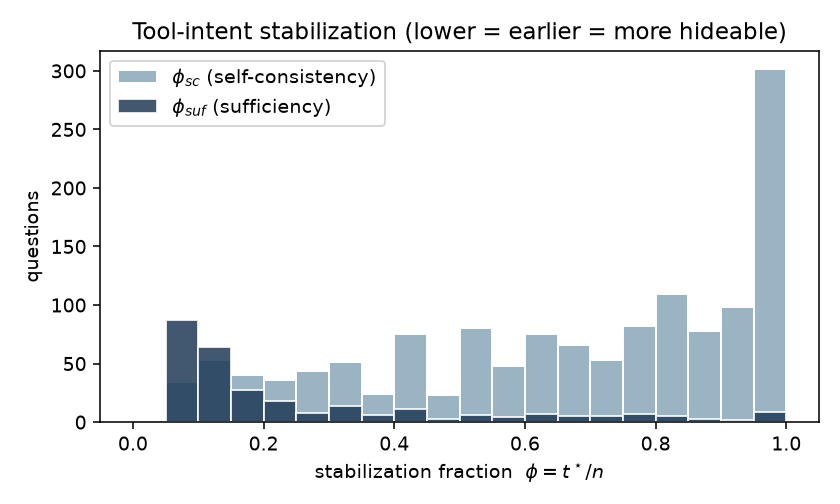
\includegraphics[width=0.78\linewidth]{figures/phi_distribution.png}
\caption{Distribution of stabilization fraction $\phi$ at $k{=}3$. Sufficiency
($\phi_{\mathrm{suf}}$, dark) concentrates near zero---gold evidence is retrievable
early---while self-consistency ($\phi_{\mathrm{sc}}$, light) is late and broad.}
\label{fig:phi}
\end{figure}

\subsection{RQ4: What predicts early vs.\ late stabilization?}
Question type is a strong predictor of $\phi_{\mathrm{suf}}$, spanning a wide range
(Table~\ref{tab:bytype}, Fig.~\ref{fig:bytype}). However, the ordering refines
hypothesis H3 rather than confirming it. H3 expected simple lookups to stabilize
early and aggregation/comparison/multi-hop to stabilize late. We instead find
\emph{aggregation} and \emph{comparison} among the \emph{earliest}-stabilizing
types, with \emph{set} questions latest. The explanation is that sufficiency
measures when the gold \emph{document} becomes retrievable, not when the answer can
be \emph{computed}: a comparison or aggregation question often names its key
entities up front, so the answer-bearing page is retrievable early even though
producing the final answer requires post-retrieval reasoning. In other words,
retrieval-sufficiency stabilization is governed by entity position in the
utterance, which is not aligned with reasoning complexity. (Several types have
small support---\texttt{set} $n{=}2$, \texttt{post-processing} $n{=}5$---so their
point estimates are noisy; the larger classes \texttt{simple}, \texttt{comparison},
and \texttt{simple\_w\_condition} are well populated.)

\begin{table}[t]
\centering
\caption{Sufficiency stabilization by CRAG question type ($k{=}3$, retrieved-gold
questions), sorted earliest to latest.}
\label{tab:bytype}
\begin{tabular}{lrr}
\toprule
question type & $n$ & mean $\phi_{\mathrm{suf}}$ \\
\midrule
aggregation          & 32  & 0.198 \\
comparison           & 59  & 0.210 \\
multi-hop            & 15  & 0.267 \\
simple               & 118 & 0.280 \\
false\_premise       & 9   & 0.289 \\
simple\_w\_condition & 52  & 0.307 \\
post-processing      & 5   & 0.310 \\
set                  & 2   & 0.658 \\
\bottomrule
\end{tabular}
\end{table}

\begin{figure}[t]
\centering
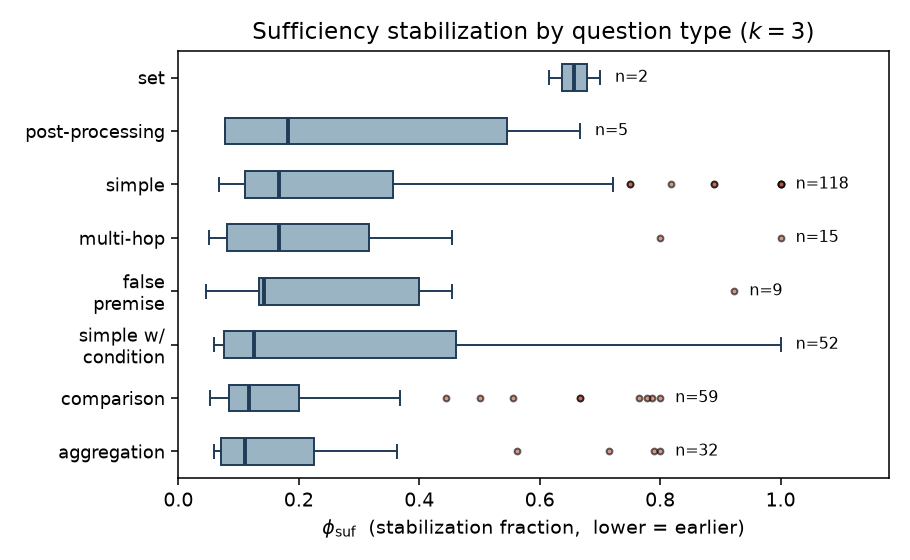
\includegraphics[width=0.92\linewidth]{figures/phi_by_type.png}
\caption{Mean $\phi_{\mathrm{suf}}$ by question type ($k{=}3$). Type spans a $3\times$
range, but the ordering tracks entity position, not reasoning complexity.}
\label{fig:bytype}
\end{figure}

\subsection{RQ2: What fraction of queries admit latency hiding?}
Using $t^\star=t_{\mathrm{suf}}$ where available and falling back to
$t_{\mathrm{sc}}$ otherwise, we compute the streamable fraction over the full
$(L,\delta,\theta)$ grid (Table~\ref{tab:rq2}, Fig.~\ref{fig:rq2}). At the central
operating point ($L{=}600$\,ms, $\delta{=}3$\,w/s, $\theta{=}0.8$), \streamPct{} of
queries admit hiding at least 80\% of tool latency. Two patterns stand out. First,
for small tool latency ($L\le300$\,ms) the constraint is essentially never binding:
$82.6\%$ of queries are streamable regardless of cadence---the residual input time
trivially covers a short tool call. Second, and confirming \textbf{H2}, when tool
latency is large ($L{=}1000$\,ms) the binding constraint becomes residual input
time, so a \emph{slower} cadence \emph{raises} the streamable fraction: from
$54.5\%$ at $\delta{=}4$\,w/s up to $73.9\%$ at $\delta{=}2$\,w/s. Faster typists
and faster talkers leave less room to hide a slow tool.

\begin{table}[t]
\centering
\caption{RQ2: streamable fraction (\%) at $\theta{=}0.8$ over the $(L,\delta)$ grid.
Rows are tool latency $L$ (ms); columns are input cadence $\delta$ (words/sec).
For large $L$, slower cadence (lower $\delta$) hides more (H2).}
\label{tab:rq2}
\begin{tabular}{lccc}
\toprule
 & $\delta{=}2$ & $\delta{=}3$ & $\delta{=}4$ \\
\midrule
$L{=}100$  & 82.6 & 82.6 & 82.6 \\
$L{=}300$  & 82.6 & 82.6 & 82.6 \\
$L{=}600$  & 82.6 & 73.9 & 73.9 \\
$L{=}1000$ & 73.9 & 63.3 & 54.5 \\
\bottomrule
\end{tabular}
\end{table}

\begin{figure}[t]
\centering
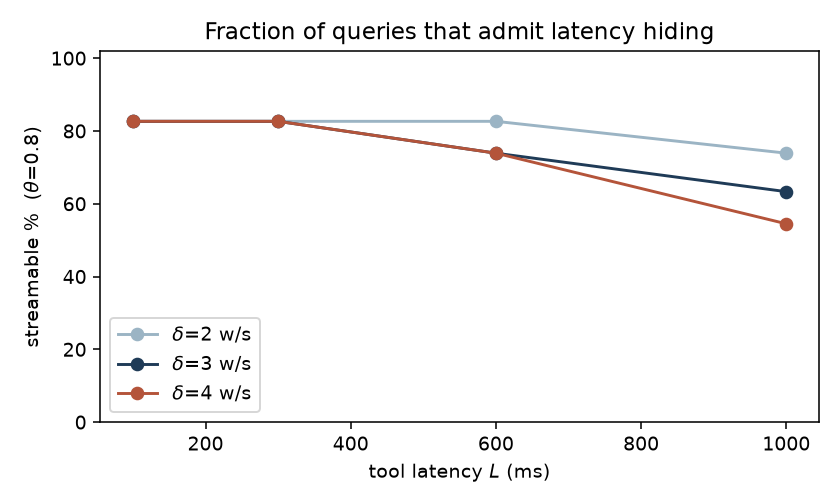
\includegraphics[width=0.78\linewidth]{figures/rq2_surface.png}
\caption{Streamable fraction vs.\ tool latency $L$ at $\theta{=}0.8$, one line per
cadence $\delta$. The curves separate only once $L$ is large enough for residual
input time to bind; there, slower cadence dominates (H2).}
\label{fig:rq2}
\end{figure}

\subsection{RQ3: Does the bound match a working pipeline?}
We replayed \rqThreeN{} retrieved-gold questions through the asynchronous Streaming
RAG harness at $L{=}600$\,ms, $\delta{=}3$\,w/s. The measured perceived-latency
saving (baseline minus streaming) averages \measSaved{}\,ms, while the $H$ bound
predicts \hPred{}\,ms (Fig.~\ref{fig:rq3}). On average, measured savings
\emph{exceed} the bound by roughly $1.9\times$ (a small number of queries where the
speculative trigger mis-fires save nothing or slightly less than baseline). This is
expected and informative:
$H$ models only the tool latency hidden behind input, whereas the calibrated
pipeline additionally overlaps the LLM's query-generation step
($\approx590$\,ms~\cite{arora2025streamrag}) with the user's input. $H$ is
therefore a \emph{conservative} predictor of realized savings---it captures the
input-hiding component and omits other overlappable costs---so a query that $H$
deems streamable will, in practice, save at least as much as predicted.

\begin{figure}[t]
\centering
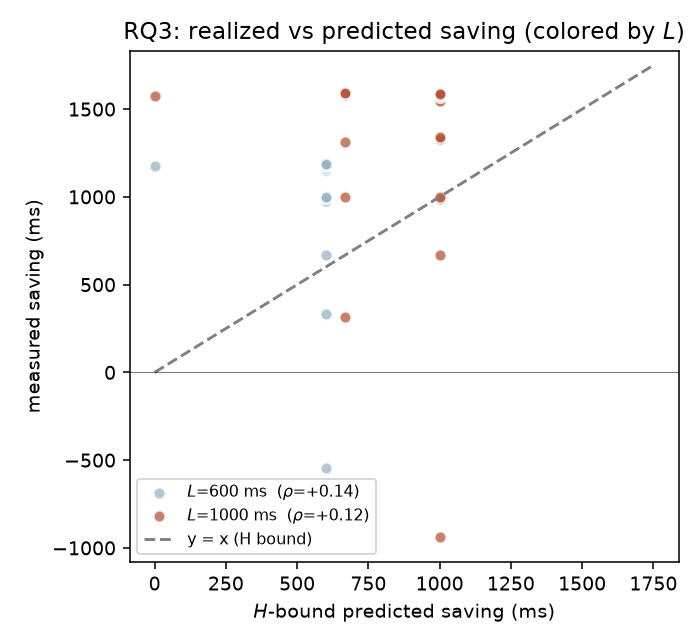
\includegraphics[width=0.5\linewidth]{figures/rq3_scatter.png}
\caption{RQ3: per-question measured saving vs.\ the $H$ bound ($\rqThreeN{}$
questions). Most points lie above $y{=}x$ because the pipeline also hides
query-generation latency, which $H$ does not model; a few queries where
speculation mis-fires show small negative savings.}
\label{fig:rq3}
\end{figure}

\subsection{Retriever robustness (top-$k$)}
Varying the sufficiency top-$k$ shifts absolute values but preserves the
qualitative picture (Table~\ref{tab:topk}). Larger $k$ surfaces the gold passage
for more questions (retrieved-gold rate $15.6\%\to25.0\%$) and stabilizes slightly
earlier (mean $\phi_{\mathrm{suf}}$ $0.327\to0.248$), as expected since a more
permissive top-$k$ is easier to satisfy. The self-consistency curve is unchanged by
$k$ (it depends only on the top-1), and the central streamable fraction is stable
near $73\text{--}74\%$. The early-sufficiency / late-self-consistency gap holds at
every $k$.

\begin{table}[t]
\centering
\caption{Top-$k$ robustness. $\phi_{\mathrm{sc}}$ (mean 0.67 / median 0.73) is
independent of $k$ and omitted.}
\label{tab:topk}
\begin{tabular}{lrrr}
\toprule
$k$ & retrieved-gold & mean $\phi_{\mathrm{suf}}$ & median $\phi_{\mathrm{suf}}$ \\
\midrule
1 & 15.6\% & 0.327 & 0.200 \\
3 & 21.3\% & 0.264 & 0.143 \\
5 & 25.0\% & 0.248 & 0.125 \\
\bottomrule
\end{tabular}
\end{table}

% ===================================================================== %

\section{Conclusion}
Tool-intent stabilization (TIS) is a query-intrinsic, model-agnostic quantity
that bounds when streaming tool use can help and by how much.  The central
finding of this paper is a measurement caution: \emph{the reported stabilization
fraction depends critically on the retrieval corpus}.  Against the per-question
candidate pool supplied by CRAG---where every document is topically relevant---
sufficiency $\phi_{\mathrm{suf}}$ is low (median \phiSufMed{} on the
retrieved-gold slice, \phiSufCleanMed{} after grounding-precision filtering),
but that pool is a favorable oracle, not the corpus a deployed system retrieves
over.  Against a realistic global corpus (NQ at ${\sim}1$M documents; FiQA at
$10\mathrm{k}$), stabilization is \emph{late}: median $\phi_{\mathrm{suf}}$
reaches \phiSufGnqOneM{} on NQ and \phiSufGfiqaBm{} on FiQA (BM25), and the
same pattern holds for dense retrieval (\phiSufGfiqaDe{} on FiQA).  These two
numbers are not in tension---they measure different operating conditions---but
practitioners must report TIS against the corpus their system actually retrieves
over.

The TIS framework itself is the durable contribution.  It provides a
principled, training-free basis for trigger design: $\phi$ and $V$ characterize
per-query stability; $H{=}\min(L,\max(0,(n{-}t^\star)/\delta))$ translates
stability into a hideable-latency budget that scales with tool latency $L$.
At small $L$ the headroom is modest regardless of corpus (\sfPqSix{} streamable
under per-question, \sfNqSix{} under global NQ at $L{=}600$\,ms); it collapses
further at large $L$ (\sfNqTwentyfive{} at $L{=}2500$\,ms) because
later stabilization leaves less residual query to overlap.  Question type gives
a significant but coarse early/late split (Kruskal--Wallis $p{=}\kwAllP{}$,
$\varepsilon^2{=}\epsSq{}$) that is preserved across retrievers
($\rho{=}\rhoDenseType{}$), providing a practical signal for selective
triggering.  The system-validation arm confirms $H$ is conservative in
aggregate ($\approx\negRateSc{}$ net-negative outcomes at $L{=}600$\,ms), and
the natural next steps---closing the per-query prediction gap and regressing
$\phi$ on linguistic features---build directly on the metrics and data released
with this paper.

\section*{Limitations}
Eight considerations bound how far the present numbers generalize; we take them
in turn, from the input model through to the retrieval corpus and benchmark.
\paragraph{Input timing.} A uniform word stream is a proxy for speech; real ASR
pacing is variable and partial hypotheses get revised. We bound this here by using
clean text and treat speech timing as planned follow-up.
\paragraph{Stabilization measure.} Top-1 equality is a coarse proxy for ``intent
settled.'' We mitigate by also reporting sufficiency against the gold document and
by varying top-$k$.
\paragraph{Grounding.} $d^\star$ is derived by string matching, so the groundable
population excludes non-verbatim answers; reported $\phi_{\mathrm{suf}}$ statistics
are conditional on groundability, and we report $t_{\mathrm{sc}}$ as a
grounding-free check.
\paragraph{Fallback population.} On the \nFallbackPct{} of queries where BM25 never
surfaces the gold passage from any prefix, stabilization is measured only by
$t_{\mathrm{sc}}$ (when the top-1 stops moving). If the top-1 in this population is
the wrong document, early settling is \emph{stable mis-retrieval}, not evidence that
the speculative query was right: $t_{\mathrm{sc}}$ certifies that intent has
\emph{stopped changing}, not that it is \emph{correct}. This is the central gap
between our measurement and end-to-end streaming-RAG quality, and it is why we keep
the sufficiency and self-consistency populations separate throughout (\S5.3) rather
than reading the blended streamable fraction as an evidence-quality claim. Our RQ3
replay finds the realized-saving and net-negative rates comparable across the two
populations at $L{=}600$ (\S5.3), but that probes \emph{perceived latency}, not
retrieval correctness, on the fallback set.

\paragraph{Per-question candidate pool.} The low $\phi_{\mathrm{suf}}$ reported
under the CRAG per-question arm (\phiSufMed{} median) is a property of the
evaluation pool, not of the retrieval problem.  CRAG supplies a small set of
topically relevant passages per question; in that oracle setting the gold
document is easy to surface from even a short prefix.  This is the source of the
v1 over-estimate: restricting to that pool inflates how early stabilization
appears to occur.  Practitioners should treat the per-question number as an
optimistic upper bound, not an operating prediction.

\paragraph{Retriever and corpus.} BM25 is lexical and phrasing-sensitive and is
known to retrieve on early topical anchors; that behavior could itself drive low
$\phi_{\mathrm{suf}}$ in the per-question arm.  We addressed this with the
dense-retriever arm (\S\ref{sec:robust}): under the per-question pool, the
bi-encoder reproduces the same low-$\phi_{\mathrm{suf}}$ pattern, confirming
the per-question result is not a BM25 artifact.  However, the global-corpus
arm---which is the correct operating condition---shows that \emph{both} BM25
and dense retrieval stabilize late (median $\phi_{\mathrm{suf}}$
\phiSufGfiqaBm{} BM25, \phiSufGfiqaDe{} dense on FiQA at $10\mathrm{k}$
distractors): the oracle artifact \emph{generalizes} to dense retrieval and
therefore does not rescue the early-stabilization claim.  The by-type ordering
is preserved across retrievers ($\rho{=}\rhoDenseType{}$), so question-type
signal remains useful for selective triggering under either retriever.

\paragraph{Global corpus scope.} The global-corpus arm uses BEIR-standard
constructions: NQ with Wikipedia passage qrels and FiQA with its finance
passage pool.  These are not the retrieval corpora of any specific deployed
system; the true operating $\phi_{\mathrm{suf}}$ is system-specific and will
depend on index size, domain, and passage granularity.  Our results establish
the direction of the corpus-size effect (later stabilization as the index
grows), but the exact number must be measured against the target system's own
index.

\paragraph{Deferred scale.} The full NQ Wikipedia passage index ($2.68$M
passages) and larger dense runs are deferred for compute reasons.  The
dose-response across $10^3$--$10^6$ distractors and the FiQA dense point at
$10\mathrm{k}$ jointly establish the trend, but the asymptotic value under a
multi-million-passage index with dense retrieval remains unmeasured.  The
present results should be read as establishing the direction and magnitude of
the corpus-size effect, not its exact operating point at deployment scale.

What remains open is cross-dataset and cross-lingual replication: a single
English QA set leaves open whether verb-final word order (e.g., Japanese or
German) shifts $t_{\mathrm{suf}}$ under lexical but not dense retrieval,
which would be a natural next step.

% \bibliographystyle is set by acl.sty; redeclaring it triggers BibTeX's
% "Illegal, another \bibstyle command" error.
\bibliography{refs}

\end{document}
